\documentclass[hyperref,UTF8]{ctexart}
\usepackage{bookmark}
\usepackage{geometry}
\geometry{a4paper,scale=0.8}
\usepackage{ctex}
\usepackage[style=caspervector,backend=biber,utf8]{biblatex}
\usepackage{booktabs}
\usepackage{array}
\usepackage{fancyhdr}
\pagestyle{fancy}
\fancyhf{}
\renewcommand\footrulewidth{1pt}
\lhead{王铠泽}
\rhead{PB18020766}
\chead{\href{mailto:volar@mail.ustc.edu.cn}{volar@mail.ustc.edu.cn}}
\rfoot{中国科学技术大学}
\lfoot{\today}
\usepackage{graphicx}
\usepackage{float}
\usepackage{subfigure}

\usepackage{hyperref}
\hypersetup{hidelinks,
	colorlinks=true,
	allcolors=black,
	pdfstartview=Fit,
	breaklinks=true
}
\begin{document}

	\centering\textbf{\LARGE{计算物理A第三次作业}}
	
	
	王铠泽\qquad PB18020766
	
		
	\section{作业题目}
	
	\begin{itemize}
		\item 在球坐标系$(r,\theta,\phi)$下产生球面上均匀分布的随机坐标点,给出其直接抽样方法。
	\end{itemize}
	
	\section{实现方法}
	
	\begin{itemize}
		\item 直接抽样法
		
		对于分布$f(\theta,\phi)$进行抽样,则有:
		$$\int_{0}^{\pi}d\theta\int_0^{2\pi}d\phi f(\theta,\phi)sin\theta =\int_{0}^{\pi}\Theta(\theta)sin\theta d\theta\int_0^{2\pi}\Phi(\phi)d\phi=1\cdot1=1$$
		
		球面的均匀分布:
		$$\int d\Omega f(\theta,\phi)=\int2\pi d\theta d\phi=1$$
		其中$\Omega$是立体角元		
		
		由上面可得:
		$$f(\theta,\phi)=\frac{1}{4\pi},\Theta=\frac{sin\theta}{2},\Phi(\phi)=\frac{1}{2\pi}$$
		
		直接抽样法:
		
		设$\xi_1,\xi_2$是$[0,1]$上生成的两组独立的伪随机数。
		则:
		$$\xi_1=\frac{\phi}{2\pi},\xi_2=\frac{1-cos\theta}{2}$$
		即:
		$$\phi=2\pi\xi_1,cos\theta=1-2\xi_2$$
		换算成直角坐标时:
	$$ \left\{
	\begin{array}{l}
	x=sin\theta cos\phi\\
	y=sin\theta sin\phi\\
	z=cos\theta\\
	\end{array} \right. $$
		\item 算法思路
			\begin{figure}[H]
				\centering
				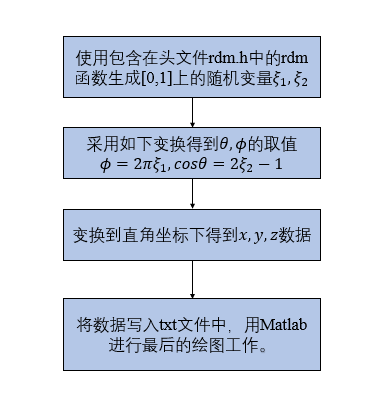
\includegraphics[width=3.3in]{intro.png}
				\caption{算法框图}\label{fig:1}
			\end{figure}
		
	\end{itemize}
	\section{程式说明}
	
	\begin{itemize}
		\item direct\_sample.c 
		
		该程式是用于生成球面上均匀分布的直接抽样程序。
		
		包含以下内容:
		\subitem rdm.h 
		
		这是一个包含了使用时间种子/默认种子的16807产生器生成随机数的头文件。
		
		\subitem void rdm(int N, double*x, int method)
		
		$method=0$ 为默认种子,$I_0=1$; $method=1$ 为时间种子生成16807的首个数据 $I_0$。
		本程序中为了保证独立性,$\xi_1,\xi_2$两个数组各自分别用默认种子和时间种子生成。
		
		\subitem int main()
		
		main函数分为两个模块,分别是生成$[0,1]$上随机序列$\xi_1,\xi_2$,得到$cos\theta,\phi$序列,得到直角坐标$x,y,z$数据并写入文件。	
		
		\item time\_seed.txt
		
		该文本文件显示的是调用时间种子时对应的原始数据。每调用一次便写入一次。检查时以最后一次生成的时间为准。
		
		\item coordinate.txt
		
		该文本文件包括了球面上均匀抽样的$(x,y,z)$数据。	
	\end{itemize}
	
	\section{计算结果}
	总点数$N=10000$,计算结果如下:
%	\begin{figure}[H]
%	\centering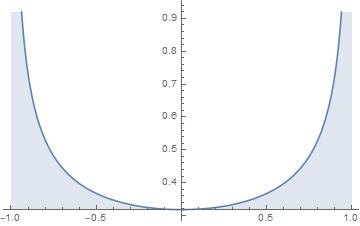
\includegraphics[width=2in]{1.jpg}
%	\caption{something}\label{fig:1}
%	\end{figure}
	
	\begin{figure}[H]
		\centering  %图片全局居中
		\subfigure[散点size=0.3 角度1]{
			\label{N=100}
			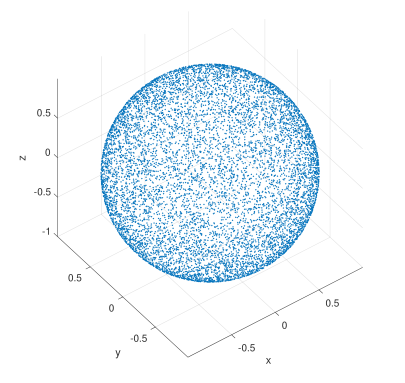
\includegraphics[width=0.45\textwidth]{../3d.png}}
		\subfigure[散点size=0.5 角度2]{
			\label{N=1000}
			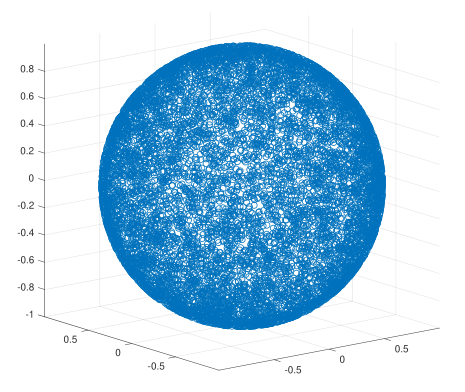
\includegraphics[width=0.45\textwidth]{../3d2.png}}
		\subfigure[散点size=0.3 x-y平面分布情况]{
			\label{N=10000000}
			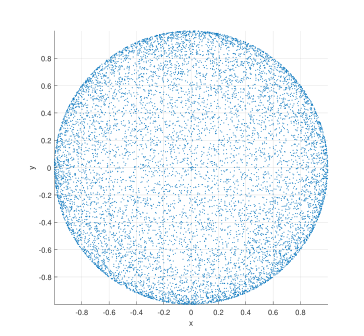
\includegraphics[width=0.5\textwidth]{../2d.png}}
		\caption{不同角度下的散点分布情况}
		\label{N}
	\end{figure}
	
	
	\begin{flushleft}
		可以看出,球面上的均匀分布投影到二维平面上体现出外围密集(边缘发散),中间稀疏的特征。这是因为在二维平面上,考虑到上下球面投影一致,有:
	
	$$g(x,y)dxdy=f(\theta,\phi)d\theta d\phi=\frac{1}{4\pi}sin\theta d\theta d\phi$$
	$$\Rightarrow g(x,y)=\frac{1}{2\pi}\vert \frac{\partial(\theta,\phi)}{\partial(x,y)}\vert=\frac{1}{2\pi}\frac{1}{\sqrt{1-r^2}}$$
	所以在二维平面上的外围会出现发散的特征。密度随着$r$增大而逐渐增大。
	
		\begin{figure}[H]
			\centering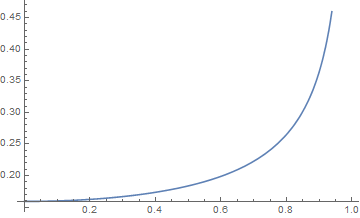
\includegraphics[width=3.5in]{../func.png}
			\caption{$g(r)$函数图像}
		\end{figure}
	\end{flushleft}
	
	
	\section{总结}
	\begin{itemize}
		\item 直接抽样法简单直观,对于简单的密度分布函数是行之有效的方法。
		\item 不同空间的"均匀"差别很大,根本原因在于度量不一样,体现在$Jacobi$行列式带来的变换因子。因此球面上的均匀嵌入到三维空间看起来不像是"均匀的"。
	\end{itemize}
	\clearpage
\end{document}